% DOCUMENT CLASS %
\documentclass[a4paper, 12pt, oneside, ngerman, twocolumn]{article}   % for A4 Paper, 12pt fontsize.
\setlength{\columnsep}{1cm}

% PACKAGES%
\usepackage{amsfonts}   % For a basic mathfont (many will be replaced by stix)
\usepackage{amsmath}    % For basic math symbols
%\usepackage{bbm}        % For \mathbbm (better version of \mathbb)
\usepackage{mathrsfs}   % For \mathscr
\usepackage{hyperref}   % For footnotes
\usepackage{csquotes}   % For \textquote{}
\usepackage{IEEEtrantools}  % For better alignments
\usepackage{tikz}   % For a macro
\usepackage{listings} % For code
\usepackage{xcolor}   % For ... code
\usepackage[babel]{microtype}
\usepackage{enumitem}
\usepackage[left=1.5cm,right=1.5cm,top=2cm,bottom=2cm]{geometry}
\usepackage{subfigure}
\usepackage[color=gray]{todonotes}
\usepackage{epigraph}   % For epigraphs
\usepackage{fancyhdr} % For headers and footers
\usepackage{cleveref} % For \cref

% To control how (section) titles look.
\usepackage{titlesec}
\titleformat{\section}
{\normalfont\Large\scshape\bfseries}
{\thesection}
{1em}
{}
\titleformat{\subsection}
{\normalfont\large\scshape\bfseries}
{\thesubsection}
{1em}
{}
\titleformat{\subsubsection}
{\normalfont\normalsize\scshape\bfseries}
{\thesubsubsection}
{1em}
{}

% Language
\usepackage[ngerman]{babel}

% If needed
\usepackage[nohyperlinks,smaller]{acronym}

% For tests
\usepackage{lipsum}

%%% FONT CONFIGURATION %%%
\usepackage{fontspec}

% Updated version of Crimson Text
\setmainfont{Cochineal}
\setmonofont{Cascadia Code}[Scale=0.8]
\usepackage[cochineal]{newtxmath} % To use Cochineal as a Math Font

% Temporary fonts when live rendering in TeXpresso
%\usepackage{newpxtext}
%\usepackage{newpxmath}
%%%

% Citing
\usepackage[style=apa, backend=biber]{biblatex}
\addbibresource{citations.bib}

% MAKE DESCRIPTION ENVIRONMENTS HAVE ITALICIZED ITEMS %
\renewcommand{\descriptionlabel}[1]{\hspace{\labelsep}\textit{#1}}

% SETS %
\newcommand*{\R}{\mathbb R}    % Set of real numbers
\newcommand*{\N}{\mathbb N}    % Set of natural numbers
\newcommand*{\Z}{\mathbb Z}    % Set of integers
\newcommand*{\Q}{\mathbb Q}    % Set of rational numbers

% BASIC CONFIGURATION %
\pagestyle{plain}
\allowdisplaybreaks

% CODE %
\definecolor{codepurple}{HTML}{7f0055}
\definecolor{comment}{RGB}{0,128,0}
\definecolor{number}{RGB}{9,136,90}
\definecolor{string}{RGB}{163,21,21}

% Things that are the same in all styles
\lstdefinestyle{basic}{
    basicstyle=\ttfamily\footnotesize,
    breakatwhitespace=false,
    breaklines=true,
    frame=leftline,
    keepspaces=true,
    numbers=left,
    firstnumber=1,
    numbersep=5pt,
    showspaces=false,
    showstringspaces=false,
    showtabs=false,
    tabsize=2,
    commentstyle=\itshape\color{comment},
    stringstyle=\color{string},
    keywordstyle=\bfseries\color{codepurple},
    texcl=true,
    mathescape=true
}

\lstdefinestyle{pseudo}{
    style=basic,
    language=python,
    morekeywords={do, od, for, if, fi, then, else, to, def, in, forall, exists, while, accept, reject},
}

\lstset{style=pseudo}


\makeatletter
\newcommand*{\textoverline}[1]{$\overline{\hbox{#1}}\m@th$}
\makeatother

\title{Wertewandel in Digitaler Kinder- und Jugendkultur \\ \large Lehrforschungsprojekt Medienpädagogik}
\date{20. November 2026}
\author{Henri Heyden \\%
    \small stu240825 \\%
    \small Christian-Albrechts-Universität zu Kiel%
}

\begin{document}

\begin{titlepage}
    \maketitle
    \thispagestyle{empty}

    \section*{Abstract}
    In diesem Lehrforschungsprojekt wird die digitale Jugend- und Kinderkultur im Zeitraum von 2008 bis 2018 analysiert.
    Dafür wird das Sprachkorpus \emph{NottDeuYTSch} verwendet, das 3 Millionen Kommentare von hauptsächlich Jugendlichen in diesem Zeitraum beinhaltet.

    Die Analyse wurde quantitativ durchgeführt, indem verschiedene computerlinguistische Algorithmen verwendet wurden, welche Lemmas zählen sowie wichtige Themen identifizieren.
    Außerdem wurde ein weiterer Algorithmus namens \emph{CorpusDiff} entworfen, um Werte-Trends in dem NottDeuYTSch Korpus auf Basis eines anderen, \emph{PoliTweets}, zu identifizieren.

    Während spaCy und BERTopic in einem überwiegend unpolitischen Datensatz wie NottDeuYTSch kaum wertbehaftete Ergebnisse liefern konnten, wurden mit CorpusDiff nachweisbare positive und negative Korrelationen mit Wertpräferenzen über die Zeit hinweg festgestellt.
    Beispielweise ergaben sich leichte positive Korrelationen zu den Themen \emph{Internationalismus} 0,167 mit 0,08\% durchschnittlichem Anstieg pro Jahr und \emph{Europa} 0,158 mit 0,1\% \dots, sowie negative Korrelationen zu \emph{Traditioneller Moral} 0,092 mit -0.034\% durchschnittlichem Abstieg pro Jahr und \emph{Verfassung} -0,069 mit -0,053\%.
    Die Korrelationen weisen eine hohe Präzision auf; die Breite des 95-\%-Konfidenzintervalls beträgt ungefähr 0,0021.

    Für zukünftige Arbeit eignet sich CorpusDiff auch, um verschiedene Korpora-Kombinationen auszuwerten.

    \subsection*{Schlüsselwörter}
    \scshape
    \hfill Kinderkultur \hfill Wertewandel \hfill NottDeuYTSch \hfill RoBERTa \hfill NLP \hfill \hfill

    \vfill
    \upshape
    \epigraph{\emph{Colorless green ideas sleep furiously.}}{Noam Chomsky, \emph{Syntactic Structures}}

    \newpage
    \thispagestyle{empty}

    \tableofcontents
\end{titlepage}

\pagestyle{fancy}
\fancyhead[L]{Wertewandel in Digitaler Kinder- und Jugendkultur \\ Lehrforschungsprojekt Medienpädagogik}
\fancyhead[R]{Henri Heyden \\ 20. November 2026}

\section{Einleitung}
Jegliche Kultur, somit auch die Kulturen, die von Kindern und Jugendlichen praktiziert werden, lässt sich zeitlich beobachten -- sie sind stets im Wandel \autocite{KWV21}.
Die Werte und Normen der \emph{Kinderkulturen} fungieren mit ihren Praktiken als hinreichende Merkmale der Kultur.
Sie definieren \emph{welche} Praktiken \emph{wie} ausgeführt werden.
Letztendlich prägen sie die späteren Erwachsenen -- die Analyse der Kinderkultur, und deren wertgeprägte Kindheitsgeschichte hat also eine wichtige pädagogische und soziologische Relevanz.

Diese Arbeit beschäftigt sich mit einem immer relevanteren Phänomen der Kinderkultur -- der digitalen Kinderkultur.

\subsection{Digitale Kinderkultur}
Seit der Digitalisierung findet viel Kinderkultur in digitalen Räumen statt.
Die Medienpädagogik beschäftigt sich außerdem viel mit Medienpraktiken und digitalen Kulturen.
Darüber hinaus werden Kind-Medien Interaktionen aus verschiedenen Blickwinkeln betrachtet.
Sie werden nicht nur im Zuge der \emph{Enkulturation} verwendet, bei der eine gewollte \emph{Erwachsenenkultur} angelernt wird.
Stattdessen erschaffen Kind-Medien Interaktionen zusätzlich sogenannte unabhängige \emph{Mikrokulturen}, die in ihren digitalen Räumen praktiziert werden.
\textcite{Sch21} beschreibt dieses Phänomen als \emph{soziomaterielle Figurationen}, die sich innerhalb der Medienpraktiken offenbaren.
Schließlich prägen diese Mikrokulturen die Erwachsenenkultur, da letztendlich Kinder mit Erwachsenen interagieren und aufwachsen.
Die moderne Pädagogik beobachtet somit in Kind-Medien Interaktionen also nicht nur eine hierarchische \emph{Lehrer-zu-Kind}-Beziehung, sondern einen flexiblen Austausch innerhalb und zwischen Generationen.
Das Phänomen, das diese Arbeit beobachtet, ist diese digitale Kinder- und Jugendkultur.

Kind-Medien Interaktionen lassen sich unter anderem direkt in ihren digitalen Räumen beobachten, um auf die Werte und Normen ihrer Mikrokulturen und dementsprechend einen Teil der digitalen Kinderkultur zu schließen.
Das Ziel dieser Arbeit ist es, genau diesen Schritt zu vollziehen -- eine Analyse der digitalen Kinderkultur und ihrer Werte auf Grundlage von Nutzerinhalten eines digitalen Raumes.

Somit definieren sich die Forschungsfragen dieser Arbeit.

\subsection{Forschungsfragen}
\paragraph{F1} Wie lässt sich die Entwicklung der digitalen Jugendkultur und ihrer Werte analysieren?
\paragraph{F2} Wie haben sich die Werte der digitalen Jugendkultur verändert?

\vspace{0.5cm}
\noindent
In dieser Arbeit werden verschiedene Techniken vorgestellt, um \textbf{F1} und \textbf{F2} mithilfe der Computerlinguistik und des Natural Language Processing (NLP) zu beantworten.

\section{Methoden und Zugänge} \label{sec:2}
Wie bereits erläutert, kann eine Kultur- bzw. Werteanalyse der digitalen Jugendkultur durchgeführt werden, indem man Inhalte, die von Jugendlichen im Internet geteilt werden, beobachtet und analysiert.
Eine andere Methode wäre auch, die Inhalte, welche Jugendliche und Kinder im Internet sehen, direkt zu analysieren.
Dies funktioniert, da die Interaktionen der Nutzer, also \emph{Likes}, \emph{Dislikes}, oder Kommentare, definieren, wie sie sich mit dem Inhalt auseinandersetzen -- stimmt der Nutzer den Inhalten/Werten eines Posts zu, oder kritisiert er/sie ihn; welche Posts mit welchen Inhalten/Werten werden öfter angesehen als andere?
Eine solche Analyse ist zum Beispiel nötig, wenn es um Plattformen geht, bei denen außer der Anzahl an \emph{Views}, keine nachweisliche Interaktion beim Post offengelegt werden kann -- in diesem Fall müssen die Inhalte selbst analysiert werden.
So ist es zum Beispiel der Fall bei \emph{YouTube Kids}, wo die Anzahl an Likes und Dislikes unter einem Video nicht öffentlich einsehbar ist, und Nutzer nicht kommentieren können.

Eine weitere Debatte ist die Art der datengestützten Analyse -- wird sie quantitativ oder qualitativ vollzogen?
Hierbei offenbart sich ein methodologischer Nachteil der direkten qualitativen Analyse von Inhalten:
Werden nur einzelne Posts und Kommentare analysiert, kann zwar für sie festgestellt werden, welche Werte sie vertreten, wie sie bei der Jugend ankommen, oder ob sie pädagogisch wertvoll sind, jedoch existiert ein Risiko, dass jene Inhalte eine unfaire Stichprobe repräsentieren, die nicht für das Gesamtbild sprechen.
Rein wissenschaftlich gesehen, könnte der Pädagoge oder die Pädagogin sogar unterbewusst Inhalte wählen, sodass seine/ihre persönliche Wertvorstellung der Kinderkultur die Analyse färbt.
Für eine Analyse der digitalen Kinderkultur ist es wichtig, ein breites Bild von Nutzerinhalten anzuschauen.

Ein Nachteil der quantitativen Analyse ist, dass sie nicht unmittelbar menschlich ausgeführt werden kann.
Wenn ein breiter Überblick der digitalen Kinderkultur gesucht wird, ist es nötig sehr viele Daten auszuwerten -- was somit nur hauptsächlich maschinell möglich ist.
Das erschwert sich dazu, dass viele digitale Plattformen heutzutage so funktionieren, dass es nur langsam möglich ist direkt Nutzerinhalte von ihrer Plattform herunterzuladen.
Die maschinelle Auswertung von Text, in diesem Fall eine Extraktion von Werten, ist zudem nicht leicht zu implementieren -- ein Computer kann zwar leicht die Syntax einer Sprache erkennen, jedoch ist es schwerer als für den Sprecher ihre Semantik zu deuten.

Ein Medium, welches von vielen Kindern und Jugendlichen weltweit verwendet wird, ist die digitale Videohosting Plattform \emph{YouTube}.
Nutzer können dort unter den meisten Inhalten, u.a. Videos, eigene Kommentare hinzufügen.
Somit ermöglicht YouTube verschiedene Kind-Medien Interaktionen, insbesondere einen Austausch von Kinderkulturen, sowie die Praktizierung von digitalen Kinderkulturen und Mikrokulturen.

\subsection{NottDeuYTSch} \label{subsec:2.1}
\emph{NottDeuYTSch} \autocite{Cot18, Cot23} ist eine Sammlung von drei Millionen YouTube Kommentaren unter Videos mit einer hauptsächlich deutschen und Jugendlichen Zuschauerschaft, zwischen 2008 und 2018.
Die Daten wurden selektiv gesammelt, um sowohl ein repräsentatives Gesamtbild der deutschen Jugendlichen YouTube Sprache darzustellen, als auch um ein Korpus zu erstellen, der vergleichbar mit anderen sei \autocite{Cot23}.

Da jeder Kommentar zeitlich indiziert wurde, können Sprach- und Wertewandel durch den Kontrast im Laufe der Zeit dargestellt werden.
NottDeuYTSch eignet sich somit hervorragend als Datenquelle, um die digitale YouTube Kinderkultur im Wandel zwischen 2008 und 2018 zu analysieren.

\subsubsection{Implementierung}
NottDeuYTSch ist in verschiedenen Formaten verfügbar unter \textcite{Cot18}.
Diese Arbeit verwendet die Version im \emph{TSV}-Format, da sie im Vergleich zu der \emph{JSON}-Variante viel kleiner ist, und somit schneller und leichter gelesen werden kann.
Für dieses Projekt wurde die Programmiersprache \emph{Python} mit der Bibliothek \emph{Pandas} verwendet, um den Umgang mit diesen großen Datensätzen zu erleichtern.

Alternativ zum TSV-Format existieren auch Formate für verschiedene linguistische Werkzeuge, wie \emph{Corpus Explorer} \autocite{Rüd22}, \emph{IMS Open Corpus Workbench} \footnote{\url{https://cwb.sourceforge.io/}}, oder \emph{Sketch Engine}\footnote{\url{https://www.sketchengine.eu/}}.
Diese Tools wurden nicht verwendet, da einerseits, es für die folgenden Ansätze leichter, schneller und effizienter war sie durch Programmierung direkt zu implementieren.
Andererseits fokussieren sich die Tools eher auf traditionelle Computerlinguistik, als auf NLP, wie es für den folgenden der Fall ist.

\subsection{RoBERTa} \label{subsec:2.2}
\emph{Cross English and German RoBERTa} \autocite{May20, RG19} ist ein Transformer KI Modell, welches verwendet werden kann, um aus englischem und deutschem Text vektorielle Einbettungen zu generieren.
Die generierten 768-dimensionalen Vektoren können mittels Winkelähnlichkeit abgeglichen werden, um eine semantische Nähe zwischen Texten zu finden.
Somit kann die Bedeutung eines Textes maschinell herausgefunden werden, indem zu verschiedenen Texten verglichen wird, bei denen eine Semantik bereits definiert ist.
Der Vorteil dieses RoBERTa Modells ist es, dass wie erwähnt sowohl englischer und deutscher Text eingebettet und verglichen werden kann -- und das mit hoher Genauigkeit \autocite{RG19}.
Solch ein bilinguales Modell ist außerdem praktisch, da ein großer Teil der deutschen Jugendsprache aus englischen Wörtern und Phrasen besteht \autocite{Po24}.

Für diese Arbeit ist ein Transformer Modell wie RoBERTa sehr nützlich, da die händische Auswertung eines großen Datensatzes wie NottDeuYTSch nahezu unmöglich ist, vollständig zu vollziehen, oder ungenau wäre, wenn man sich auf eine evaluierbare Teilmenge beziehen würde.

\subsubsection{Implementierung}
In Python kann die \emph{sentence transformers} Bibliothek \autocite{RG19} verwendet werden, um Modelle wie RoBERTa von der \emph{Hugging Face}\footnote{\url{https://huggingface.co/}} Plattform herunterzuladen und einzubinden.
Ein weiteres Feature dieser Bibliothek ist es, dass Modelle auf der Grafikkarte ausgeführt werden können, was die Berechnungen erheblich beschleunigt, da somit viele Berechnungen parallel ausgeführt werden können.

Nichtsdestotrotz war die vollständige Einbettung von NottDeuYTSch sehr aufwändig und erforderte 30 Minuten Rechenzeit.
Die 768-dimensionalen Vektoren wurden als Felder vom Typ \lstinline|float32| gespeichert, was bei der Menge an 3 Millionen Vektoren in ungefähr 9,2 Gigabyte Speicherverbrauch resultierte.
Aus diesem Grund habe ich die Schritte der folgenden Pipeline vollständig modular implementiert, sodass Zwischenergebnisse gespeichert werden, bevor der nächste Schritt ausgeführt wird.

\subsection{PoliTweets} \label{subsec:2.3}
\textcite{Bie22} präsentiert \emph{PoliTweets} -- einen Datensatz aus zehntausenden deutschen Posts der Social-Media-Plattform \emph{X}, ehemals \emph{Twitter}.
Einzelne \emph{Tweets} wurden dabei mit verschiedenen Labels ausgezeichnet, die eine politische Gesinnung zu einem bestimmten Thema darlegen.

PoliTweets eignet sich aus vielen Gründen sehr gut für diese Arbeit.
Erst mal, da es aus nur aus deutschsprachigen Texten im Online-Lingus besteht, jedoch auch, da zwölf der Kategorien sowohl positive als auch negative Beispiele erhalten.
Letzteres ist sehr wichtig, da RoBERTas 768-dimensionale Vektoren nicht nur die \emph{Aussage} eines Textes kodieren, sondern auch ihren \emph{Stil}, also die Art von Sprache im Text.
Dementsprechend würde eine Metrik, die beispielsweise Progressivität misst auf Basis der Winkelähnlichkeit zu \emph{progressiven} Texten, zum größten Teil nur die stilistische Nähe zu der Sprache im Datensatz der progressiven Texte messen.
Dieses Phänomen nennt man auch Störfaktor oder eng. \emph{Confounder}.

Mithilfe von positiven und negativen Labels zu einzelnen Themen, kann man stattdessen eine Metrik definieren, basierend auf der Differenz der Winkelähnlichkeit zu positiven und negativen Beispielen.
Formaler, sei \(\lambda : V^2 \rightarrow [-1, 1], (v, w) \mapsto \frac{v \cdot w}{||v|| \cdot ||w||}\) die Kosinus-Winkelähnlichkeit zwischen Vektoren \(v, w\) im verwendeten Vektorraum\footnote{Ist der Vektorraum \(V\) normalisiert, also haben alle Vektoren Länge eins, kürzt sich die Division durch das Produkt der Längen, was erheblich die Berechnung effizienter macht.} \(V \subseteq [-1, 1]^{768}\).
Außerdem, seien \(P_l, N_l, \Omega \subseteq V\) paarweise disjunkt.
\(P_l\) und \(N_l\) stellen die positiven und negativen Einbettungen aus PoliTweets zu einem Thema \(l\) dar, während \(\Omega\) die Menge der Einbettungen aus NottDeuYTSch ist.
Die \(l\)-Metrik \(\alpha_l : \Omega \rightarrow [-1, 1]\) ist definiert durch
\begin{IEEEeqnarray*}{c}
    \alpha_l: v \mapsto \frac{\sum_{u \in P_l} \lambda(v, u)}{2|P_l|} - \frac{\sum_{u \in N_l} \lambda(v, u)}{2|N_l|}.
\end{IEEEeqnarray*}
In anderen Worten, \(\alpha_l(v)\) ist die Differenz zwischen der durchschnittlichen Ähnlichkeit zu positiven und negativen Texten über Thema \(l\).
Durch diesen Ansatz umgeht man das Problem, dass \(\lambda\) zwischen \(\Omega\) und \(P_l\) eben nicht nur \(l\) misst, sondern auch die stilistische Nähe zu Texten aus PoliTweets.

Zu dieser Methode ist zu beachten, dass nicht einzelne Werte dieser Metrik zu interpretieren sind, sondern ein Durchschnitt vieler im zeitlichen Verlauf.
Außerdem ist sie nur so akkurat, wie der Vergleichskorpus genau ist, und möglichst viele positive und negative Beispiele für \(l\) enthält.

\subsubsection{Implementierung}
Die Implementierung der \(l\)-Metrik bestand daraus Einbettungen für alle Texte aus PoliTweets zu erstellen, bei denen das Label eines der zwölf Kategorien gleicht, die sowohl positive als auch negative Beispiele enthalten.
Bei der eigentlichen Berechnung ergab sich ein weiterer Vorteil der sentence transformers Bibliothek, da auch die Winkelähnlichkeit zwischen Vektoren effizient auf der Grafikkarte parallelisiert berechnet werden kann.
An Rechenzeit erforderte die Berechnung der Winkelähnlichkeiten somit nur eine Minute.

\subsection{CorpusDiff}
Die kombinierte Methode, die ich in \cref{subsec:2.1,subsec:2.2,subsec:2.3} beschrieben habe, nenne ich \emph{CorpusDiff}.
Siehe \autoref{fig:1} für eine Illustration der Pipeline.
Ein Vorteil dieser Methode ist es, dass sie auf alle möglichen Kombinationen von Sprachkorpus, gelabelten positiven/negativen Vergleichskorpus und Transformer anwendbar ist -- sie lässt sich also verwenden, um beliebige feste Trends und Wandel in jeglichem Korpus zu identifizieren.

\begin{figure}
    \centering
    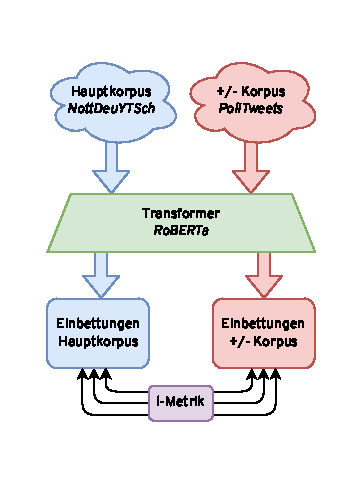
\includegraphics[width=0.4\textwidth]{./figures/Pipeline.pdf}
    \caption{Der Aufbau von CorpusDiff um \(l\)-Metriken für einen Sprachkorpus zu berechnen.}
    \label{fig:1}
\end{figure}

\subsection{Lemmatisierung \& Bag-of-Words} \label{subsec:2.5}
Eine sehr simple, konservative Methode der Computerlinguistik basiert auf der Lemmatisierung von Wörtern.
Hierbei wird ein Wort auf eine Grundform, ein \emph{Lemma}, reduziert, welches die Bedeutung des Wortes repräsentiert.
Zum Beispiel wäre das Lemma von \emph{lief} das Verb \emph{laufen}, oder jeglicher Artikel in jeglichem Kasus wird zu \emph{der} umgewandelt.

Im Gegensatz zur Wortstammfindung, wo ein Lexem kontextfrei in seine Urform umgewandelt wird, behält die Lemmatisierung die Semantik aus dem Kontext.
Beispielweise produziert das Wort \emph{Maus} ein unterschiedliches Lemma, je nachdem ob das Tier oder die Computermaus gemeint ist.
Dementsprechend ist Lemmatisierung nicht eine triviale Aufgabe wo nach einer endlichen Menge an Regeln ein Wort auf eine Grundform reduziert wird.

Durch Lemmatisierung können einzelne Kommentare in Listen an Lemmas umgewandelt werden.
Dabei werden einige unnötige Worttrenner, wie Leerzeichen, Ausrufezeichen, oder \lstinline|:D| aus dem Text entfernt.
Die nun generierten Lemmas können mithilfe von simplen Algorithmen analysiert werden.
Ein möglicher Algorithmus ist ein sog. \emph{bag-of-words} Algorithmus, bei dem einfach Wortzahlen gezählt werden.
Davor kann es außerdem zum Vorteil sein, allgemeine unwichtige Wörter hinauszufiltern.
Eine Methode dies zu tun ist es, eine Menge an sog. \emph{Stoppwörtern} aus den Listen von Lemmas zu entfernen.

Verschiedene Wörter haben unterschiedliche Bedeutungen, und können verschiedene Werte repräsentieren.
Zwar verschwindet der Kontext, in dem das Lemma verwendet wurde, jedoch impliziert seine Popularität die relative Relevanz des Diskurses über den Wert, den es repräsentiert.

\subsubsection{Implementierung}
Mittels der Python Bibliothek \emph{spaCy} \autocite{HMVB20} können Transformer Modelle verwendet werden, um Texte zu lemmatisieren.
Dazu bietet spaCy das \lstinline|de_core_news_sm|\footnote{\url{https://spacy.io/models/de\#de_core_news_md}} Modell an, welches wie RoBERTa, Einbettungen von Texten produziert.
Der relevante Unterschied ist jedoch, dass spaCy einzelne Lexeme, bzw. \emph{Tokens}, einbettet, und nicht ganze Sätze.

spaCy bietet leider keine Methode an, die Lemmatisierung auf meiner Grafikkarte zu beschleunigen.
Jedoch ist es möglich durch sog. \emph{Batching} die Lemmatisierung des ganzen Korpus auf viele kleine Abschnitte aufzuteilen.
Die einzelnen \emph{Batches} können effizient auf den Kernen der CPU parallelisiert lemmatisiert werden.
Bei meinem Ryzen 9 5950X Prozessor dauert die Lemmatisierung mit dieser Methode ungefähr 15 Minuten.

Um die Stoppwörter zu entfernen wurde die \emph{stopwordsiso}\footnote{\url{https://pypi.org/project/stopwordsiso/}} Bibliothek verwendet.
Außerdem wurden alle Lemmas in Kleinbuchstaben umgewandelt, um doppelte Lemmas wie \emph{geil} und \emph {Geil} zusammenzuschließen.
Für die Wordcloud wurden des Weiteren alle Lemmas mit Länge eins nicht beachtet, um die meisten Emojis zu entfernen.
Das Zählen selber ist recht leicht zu implementieren, und braucht nicht viel Laufzeit.

\subsection{BERTopic}
BERTopic \textcite{Gro22} ist ein sog. \emph{neural topic modeling} (NTM) \autocite{Wu24} Ansatz der verwendet werden kann, um die relevantesten Themen aus einer Sammlung von Texten zu finden.
BERTopic ist modular aufgebaut und besteht aus den folgenden Schritten.
\begin{enumerate}
    \item Vektorielle Einbettung des Korpus: \\
        Zuerst werden mittels eines Transformers Vektoren von einzelnen Texten erstellt.
        Dazu lässt sich RoBERTa direkt verwenden.

    \item Dimensionsreduktion des Vektorraums: \\
        BERTopic verwendet verschiedene Techniken, wie zum Beispiel UMAP \autocite{MHM20}, um die Dimension des Vektorraums so zu reduzieren, dass so wenig wie möglich relevante Informationen verloren gehen.

    \item Clustering der Vektoren: \\
        Nun werden Gruppen, sog. \emph{Cluster}, innerhalb des Vektorraums gefunden -- konzentrierte Strukturen von Vektoren, die verschiedene Themen repräsentieren.
        Dieser Schritt erfolgt meistens mit dem HDBSCAN \autocite{MB19} Algorithmus.

    \item Cluster Namen Generierung: \\
        Zuletzt werden allen Clustern Namen zugeordnet, die den jeweiligen Cluster repräsentieren -- dem \emph{Topic}.
        BERTopic verwendet dabei einen bag-of-words Ansatz, bei dem der Name eines Clusters aus den häufigsten Wörtern generiert wird, welche selten in anderen Clustern vorkommen.
\end{enumerate}
Somit können mittels BERTopic ähnliche Ergebnisse wie mit dem vorherigen Ansatz erreicht werden.
Der wichtige Unterschied ist jedoch, dass der Kontext im gesamten Kommentar wichtig ist für seine Bedeutung, wobei der Lemmatisierung nur die Bedeutung einzelner Wörter ermittelt wird.
BERTopic ist sozusagen eine raffiniertere Version des klassischen bag-of-words Ansatzes.

\subsubsection{Implementierung}
BERTopic kann über die \emph{bertopic}\footnote{\url{https://pypi.org/project/bertopic/}} Python Bibliothek eingebunden werden.
Da die RoBERTa Einbettungen von NottDeuYTSch zuvor zwischengespeichert wurden, musste nicht ein weiteres Mal das Korpus eingebettet werden -- die Vektoren konnten direkt an BERTopic weitergegeben werden.
Für die Dimensionsreduktion wurde UMAP verwendet, und HDBSCAN wurde zum Clustern angewendet.

BERTopic ermöglicht außerdem die Berechnung der Wahrscheinlichkeiten, wie sicher ein Thema zu einem Text passt.
Allerdings resultiert dies in extremen Arbeitsspeicherverbrauch.
Da auf meiner Maschine nur 32 Gigabyte RAM zur Verfügung stehen, musste ich auf \emph{Swapping} zurückgreifen, was die Performance insgesamt so verlangsamt hatte, dass das Programm nicht innerhalb sechs Stunden terminierte, und ich abbrechen musste.

Wenn die Wahrscheinlichkeiten nicht berechnet werden sollen, kommt man mit meinem Setup stattdessen auf ungefähr zwei Stunden Rechenzeit.

\subsection{Zusammenfassung}
Generell lassen sich somit die in \autoref{sec:2} erwähnten Ansätze in drei Methoden aufteilen:
\begin{enumerate}
    \item Lemmatisierung mit spaCy \lstinline|de_core_news_sm| Modell, und dann Worte zählen, gegebenenfalls eine Wordcloud erstellen und zuletzt händisch populäre Wörter durchgehen, um Werte(-Trends) nachzuweisen.

    \item Anwendung von BERTopic, um dann die generierten Topic-Namen durchzugehen, und ähnlich wie bei der Lemmatisierung nach Werte(-Trends) zu Suchen.

    \item CorpusDiff: Einbettung von NottDeuYTSch und PoliTweets mittels RoBERTa, Berechnung und statistische Auswertung aller \(l\)-Metriken, siehe \autoref{subsec:2.3}.
\end{enumerate}
Im Folgenden werden die Ergebnisse dieser drei Ansätze präsentiert.

\section{Ergebnisse}
Die Ergebnisse der Analyse von NottDeuYTSch lassen sich in ihre drei Methoden gliedern.

\subsection{Lemmatisierung \& Bag-of-Words}
Schaut man sich die Wordcloud generiert aus allen Lemmas nach \autoref{subsec:2.5} an, siehe \autoref{fig:2}, sieht man ein ernüchterndes Ergebnis:
Man sieht direkt, dass, selbst wenn alle Stoppwörter herausgefiltert werden, der Großteil wenig mit Werten zu tun hat, sondern viel mehr die jugendliche YouTube-Kultur betont.
\citeauthor{Sch21}s soziomaterielle Figurationen kommen wieder zum Vorschein -- der absolute Mehrheit der Kommentare setzen sich mit dem Inhalt oder der Plattform und ihren Medienpraktiken auseinander.

\begin{figure}
    \centering
    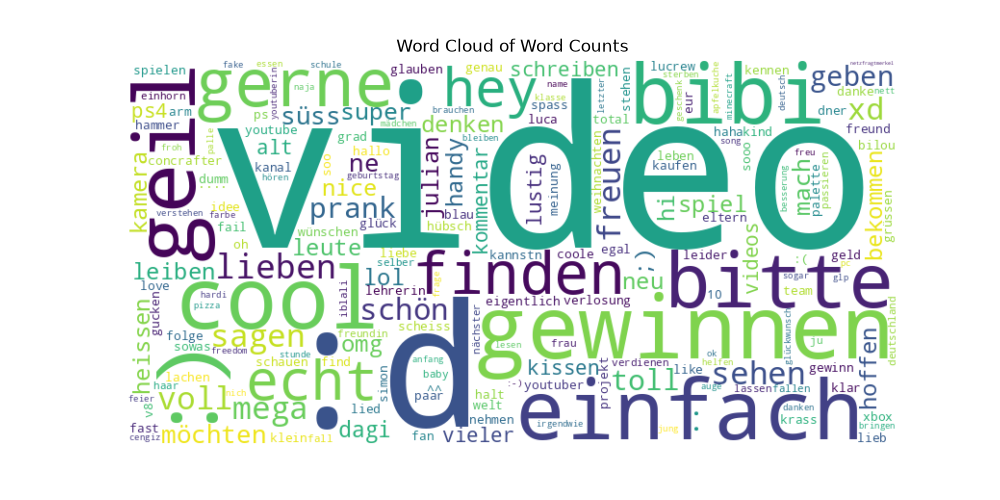
\includegraphics[width=0.5\textwidth]{./figures/wordcloud/wc.png}
    \caption{Die Wordcloud generiert aus dem gesamten NottDeuYTSch Korpus.}
    \label{fig:2}
\end{figure}

Um etwas tiefer zu schauen, wurde eine Tabelle mit allen Wortzählungen erstellt, und sie nach Häufigkeit sortiert.
Leider wurden in dieser Tabelle im Vergleich zu wenig Stichwörter gefunden, mit deren temporäre Häufigkeit eine akkurate Werteanalyse weitergeführt werden hätte können.
Um dies zu demonstrieren ist ein Teil der Wortzählung in \autoref{tab:1} zu finden.
Das Wort \emph{woke} kommt sogar kein mal im gesamten Korpus vor.

\begin{table}
    \centering
    \begin{tabular}[c]{l l}
        \hline
        Lemma & Frequenz \\
        \hline \hline
        Video & 280975 \\
        Gewinnen & 128772 \\
        Cool & 122297 \\
        Deutschland & 13278 \\
        Nazi & 2370 \\
        Gleichberechtigung & 509 \\
        Feminismus & 186 \\
        Vielfalt & 45 \\
        Emanzipation & 28 \\
        Inklusion & 12 \\
        Woke & 0 \\
        \hline
    \end{tabular}
    \caption{Auszug der gesamten Wortzählung im lemmatisierten NottDeuYTSch.}
    \label{tab:1}
\end{table}

Diese Methode wäre in einem politischem Korpus besser geeignet gewesen, jedoch wurde während der Recherche leider kein solcher Korpus gefunden.
Andererseits muss betont werden, dass jegliche Wortzählung sich auf nur den Kontext eines Wortes bezogen werden kann.
Dementsprechend geht Ironie verloren, wenn sie in einem Kommentar angewandt wird: \emph{Das war lustig....nicht. sry} -- User Hoshi82.

Ein ähnlicher Ansatz wäre es sog. \emph{N-Gramme} zu finden, bei denen jeweils nach \(n \in \N\) langen Lexemkombinationen gesucht werden -- die klassische Wortzählung ist die Suche nach 1-Grammen.
Jedoch verliert man Häufigkeiten je größer \(n\) ist.
Außerdem lässt sich Ironie oder ein Widerspruch auch in einem Satz so verkapseln, dass man sie erst finden kann, wenn erst der vollständige Satz interpretiert wird: \emph{Ich bin ein Teil von jener Kraft, die stets das Böse will und stets das Gute schafft}.

\subsection{BERTopic}
Für den Ansatz mit BERTopic kamen ähnliche Ergebnisse heraus, wie mit dem klassisch-linguistischem bag-of-words Ansatz -- die meisten Themen, die von BERTopic identifiziert wurden, haben mit Videoinhalten oder dem Medium YouTube zu tun.
Andererseits wurden trotzdem interessante Themen gefunden, siehe \autoref{tab:2}.

\begin{table}
    \centering
    \begin{tabular}[c]{l l}
        \hline
        Name des Themas & Frequenz \\
        \hline \hline
        \emph{Kein Thema} & 1232594 \\
        lehrer\_lehrerin\_schüler\_unterricht & 9155 \\
        apfelkuchen\_\dots\_äpfelkuchen & 7761 \\
        lustig\_witzig\_humor\_funny & 7225 \\
        pc\_gtx\_ram\_i7 & 6629 \\
        freedom\_folgen\_projekt\_folge & 3862 \\
        dumm\_blöd\_dummheit\_stupid & 3789 \\
        \hline
    \end{tabular}
    \caption{Auszug der Frequenz mit BERTopic gefundener Themen in NottDeuYTSch.}
    \label{tab:2}
\end{table}

Aus dieser Tabelle offenbaren sich mehrere Probleme:
\begin{enumerate}
    \item Es wurden zu wenig relevante politische Themen gefunden.
    \item BERTopic ordnet jedem Kommentar nur ein Thema zu.
    \item Einer sehr großen Minderheit an Kommentaren wurde kein Thema zugeordnet.
\end{enumerate}
Das erste Problem erklärt sich dadurch, dass, wie bereits erläutert, der Korpus hauptsächlich unpolitisch ist.
Das zweite und dritte Problem sind methodische Fehler in der Implementierung von BERTopic.
Allerdings muss dabei bedacht werden, dass wenn ein Kommentar mehreren/mindestens einem Thema zugeordnet werden soll, sich die bereits unvorteilhafte Laufzeit bei der Menge an Daten maßgeblich verschlechtert.
Dementsprechend ist es mit einem Ansatz wie dem von BERTopic sehr unwahrscheinlich eine sehr genau Analyse zu finden.

Mit den Daten, die wir nun haben lassen sich nichtsdestotrotz Trends identifizieren.
Um diese Analyse durchzuführen, habe ich die relevanten Themen aus \autoref{tab:2} im Zeitraum 2008 bis Ende 2018 visualisiert, siehe \autoref{fig:3}.
Für diese Abbildung wurden erst alle Kommentare in alle einzelnen Monate aufgeteilt und durch die Anzahl an Kommentaren in diesem Monat geteilt, um relative Häufigkeiten zu berechnen.
Zudem wurde ein sog. \emph{rolling window} Filter benutzt, der in einem Fenster von den 2 umliegenden Jahren die oberen und unteren 25\% entfernt, und den Durchschnitt berechnet.
Dies hatte den Grund, da bei der im Vergleich geringen Menge an Kommentaren zu einem Thema zu der Menge an einzelnen Monaten, die meisten Kommentare keinen Kommentar zu einem Thema besitzen.
Andererseits haben die Monate, die mindestens einen Kommentar zu jenem Thema besitzen, besonders viele.
Dies war besonders bei den Themen \emph{Apfelkuchen} und \emph{Lehrer} der Fall, da NottDeuYTSch anscheinend ein paar Videos zu genau diesen Themen gewählt hatte, die natürlich dementsprechend nur aus Kommentaren über diese Themen bestanden.
Zuletzt gab es auch ein weiteres Problem, das sich schon in \autoref{tab:2} finden ließe:
es gab zwischen verschiedenen Themen erhebliche Unterschiede der Größenordnungen.
Dies wurde gelöst, indem die Y-Achse logarithmisch skaliert wurde, wodurch sowohl größere als auch kleinere Unterschiede sichtbar werden.
Im Quellcode zu dieser Arbeit lässt sich genaueres dazu finden, siehe Anhang.

\begin{figure}
    \centering
    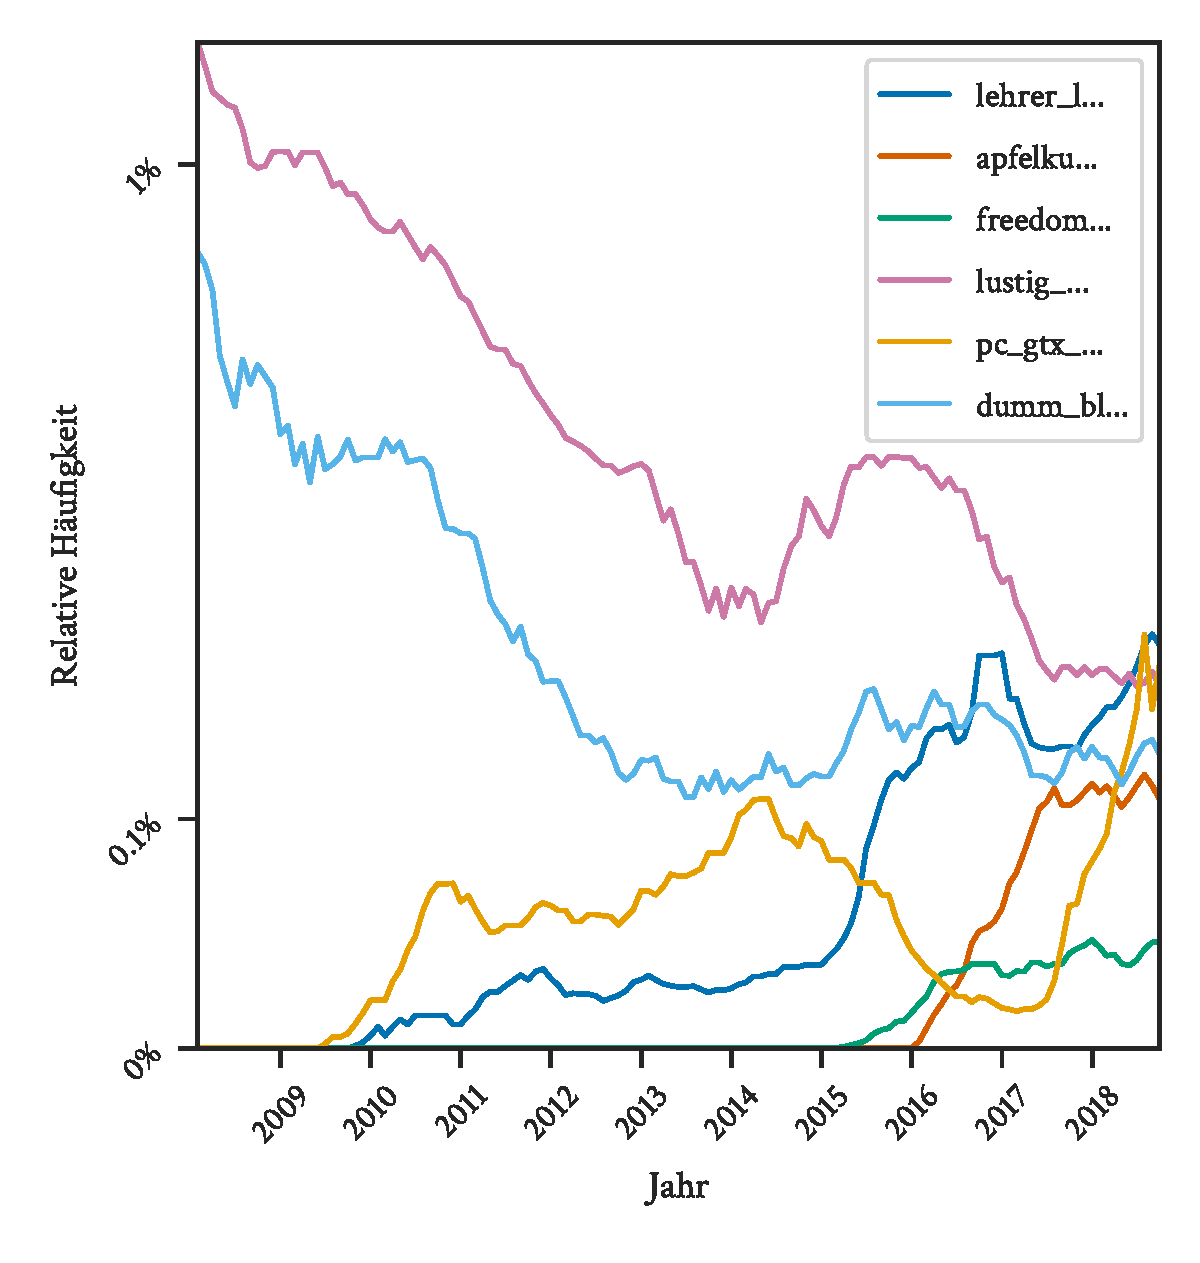
\includegraphics[width=0.45\textwidth]{./figures/Bertopic.pdf}
    \caption{Mittels BERTopic identifizierte Trends in NottDeuYTSch.}
    \label{fig:3}
\end{figure}

Aus der Abbildung lässt sich interpretieren, dass es einen negativen Trend zu humoristischen und direkt beleidigenden Kommentaren gab.
Daraus einen Werte-Trend zu identifizieren ist jedoch nicht trivial.
Es ließe sich vermuten, dass diese sich Trends durch eine Veränderung des Mainstreams erklären.
Ein Indiz dafür wäre die Entwicklung der Meme-Kultur, die besonders 2008 sehr durch \emph{rage comics} wie dem sog. \emph{Trollface} oder absurden Kurzvideos wie \emph{ASDFMovie}\footnote{\url{https://youtu.be/meR20w6MiUc}} gesättigt war.

\subsection{CorpusDiff}
Die um die Ergebnisse der \(l\)-Metriken auszuwerten, wurden Pearson-Korrelation-Koeffizienten \autocite{Ber18} berechnet und ein linearer \emph{least-squares} Regressor \autocite{Baz21} gefittet, um die durchschnittliche Steigung, also den durchschnittlichen Zuwachs/Abfall der \(l\)-Metrik in einem Jahr zu bestimmen.
Diese Daten sind in \autoref{tab:3} zu finden.

\begin{table*}
    \centering
    \begin{tabular}[c]{lrrr}
        \hline
        \(l\)-Metrik & Korrelation & 95\%-Konfidenzintervall & Durch. Jahresanstieg \\
        \hline
        \hline
        traditional morality & -0.092 & (-0.093, -0.091) & -0.034\% \\
        constitution & -0.069 & (-0.070, -0.067) & -0.053\% \\
        education & -0.060 & (-0.061, -0.059) & -0.062\% \\
        protectionism & -0.060 & (-0.061, -0.059) & -0.031\% \\
        foreign special & -0.039 & (-0.040, -0.038) & -0.066\% \\
        welfare & -0.035 & (-0.036, -0.034) & -0.005\% \\
        multiculturalism & -0.001 & (-0.002, -0.000) & -0.031\% \\
        labour & 0.077 & (0.076, 0.078) & 0.081\% \\
        military & 0.116 & (0.115, 0.117) & 0.018\% \\
        national way of life & 0.147 & (0.146, 0.148) & 0.036\% \\
        europe & 0.160 & (0.159, 0.162) & 0.100\% \\
        internationalism & 0.169 & (0.168, 0.170) & 0.080\% \\
        \hline
    \end{tabular}
    \caption{Pearson-Korrelation-Koeffizienten und durchschnittliche Steigung aller \(l\)-Metriken.}
    \label{tab:3}
\end{table*}

Des Weiteren wurden zwei Visualisierungen erstellt, die jeweils den zeitlichen Verlauf aller \(l\)-Metriken direkt, siehe \autoref{fig:4}, sowie Z-standardisiert \autocite{BD07}, siehe \autoref{fig:5}, abbilden.
Da für jeden Kommentar alle \(l\)-Metriken berechnet werden, existieren für einzelne Monate offenbar sehr viele Datenpunkte, was eine Visualisierung erschwert.
Wie in der Visualisierung für BERTopic wurde deshalb der gleiche rolling window Filter angewendet, um Rauschen zu verhindern, und die einzelnen Metriken besser vergleichbar zu machen.
Des Weiteren wurden für \autoref{fig:4} eine obere und untere Schranke nahe der 25\%- und 75\%-Quartile eingefügt, um die starke Varianz abzubilden.

\begin{figure*}
    \centering
    \begin{subfigure}
        \centering
        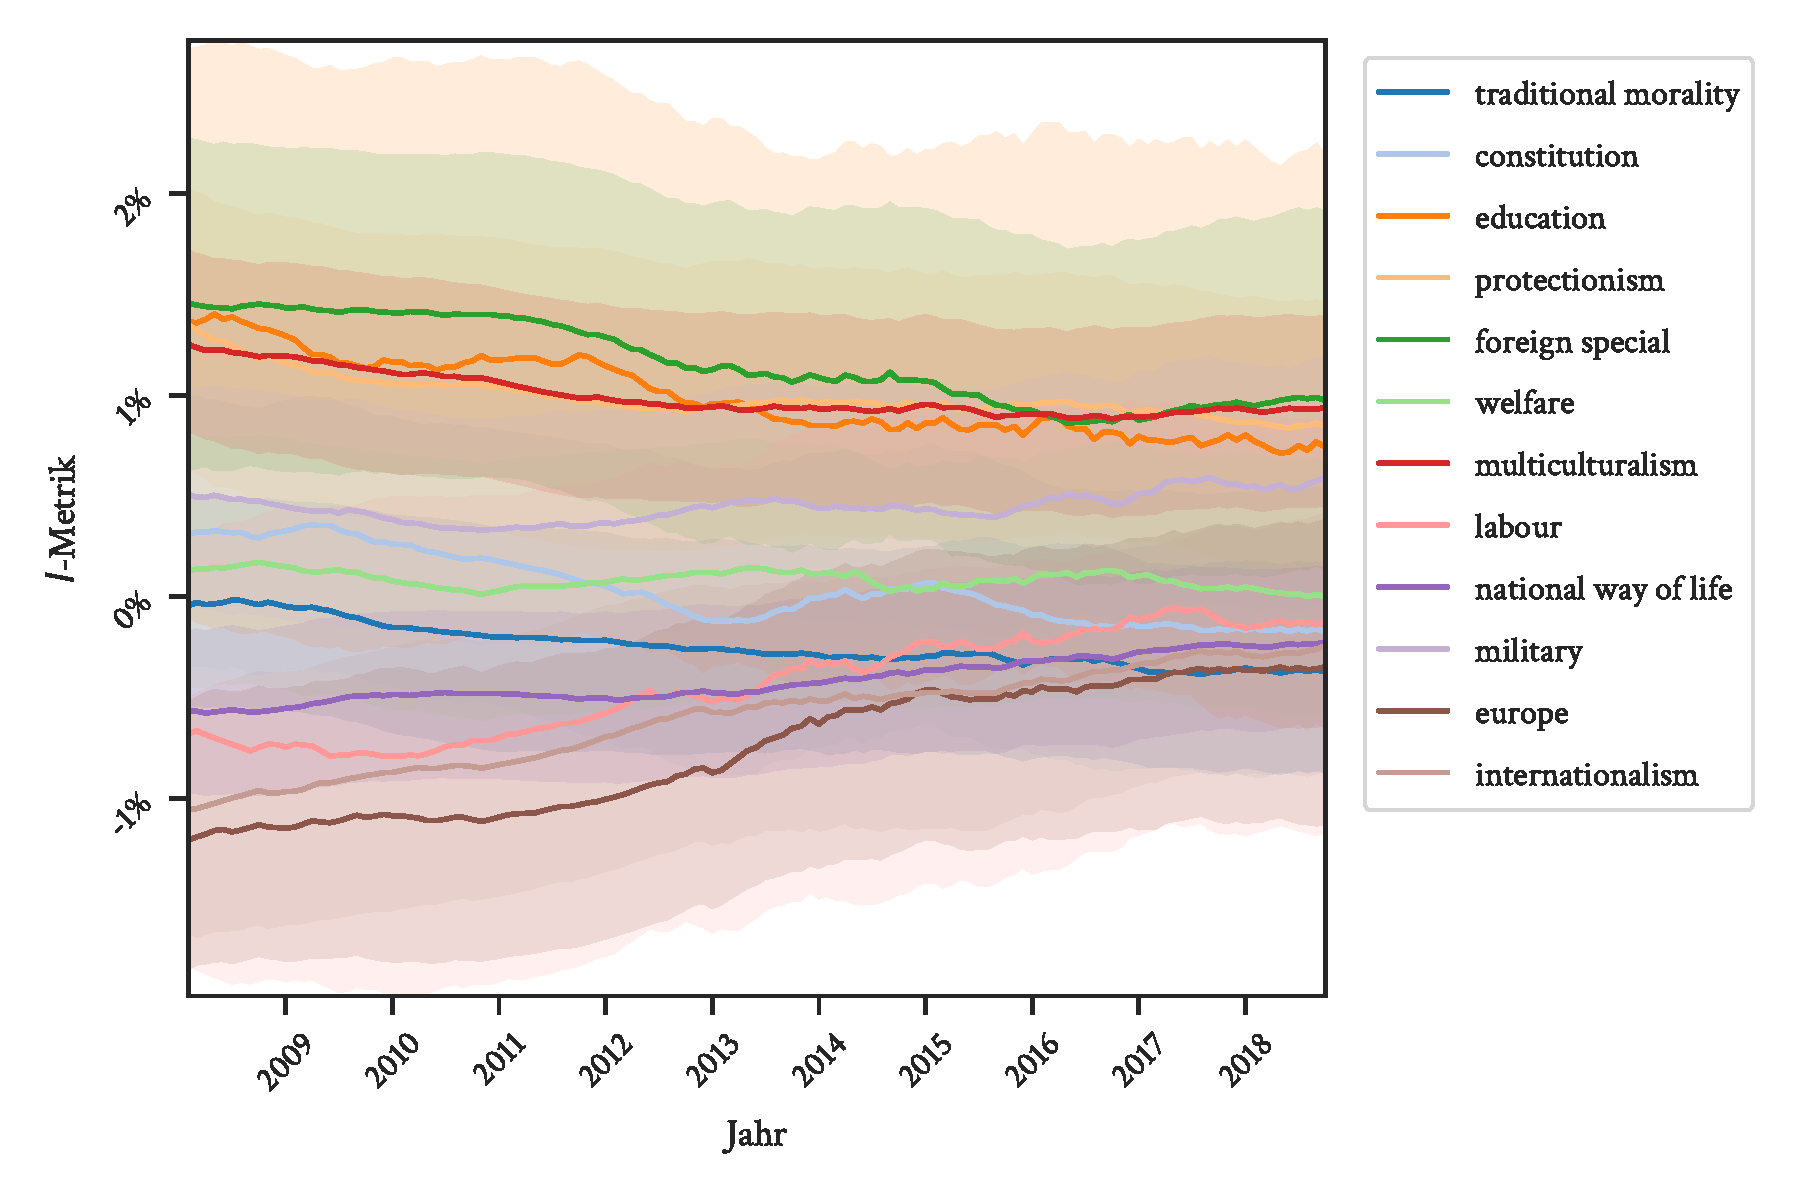
\includegraphics[width=0.9\textwidth]{./figures/lmetric_filtered.pdf}
        \caption{\(l\)-Metriken mit durchschnittlichem Spektrum.}
        \label{fig:4}
    \end{subfigure}

    \begin{subfigure}
        \centering
        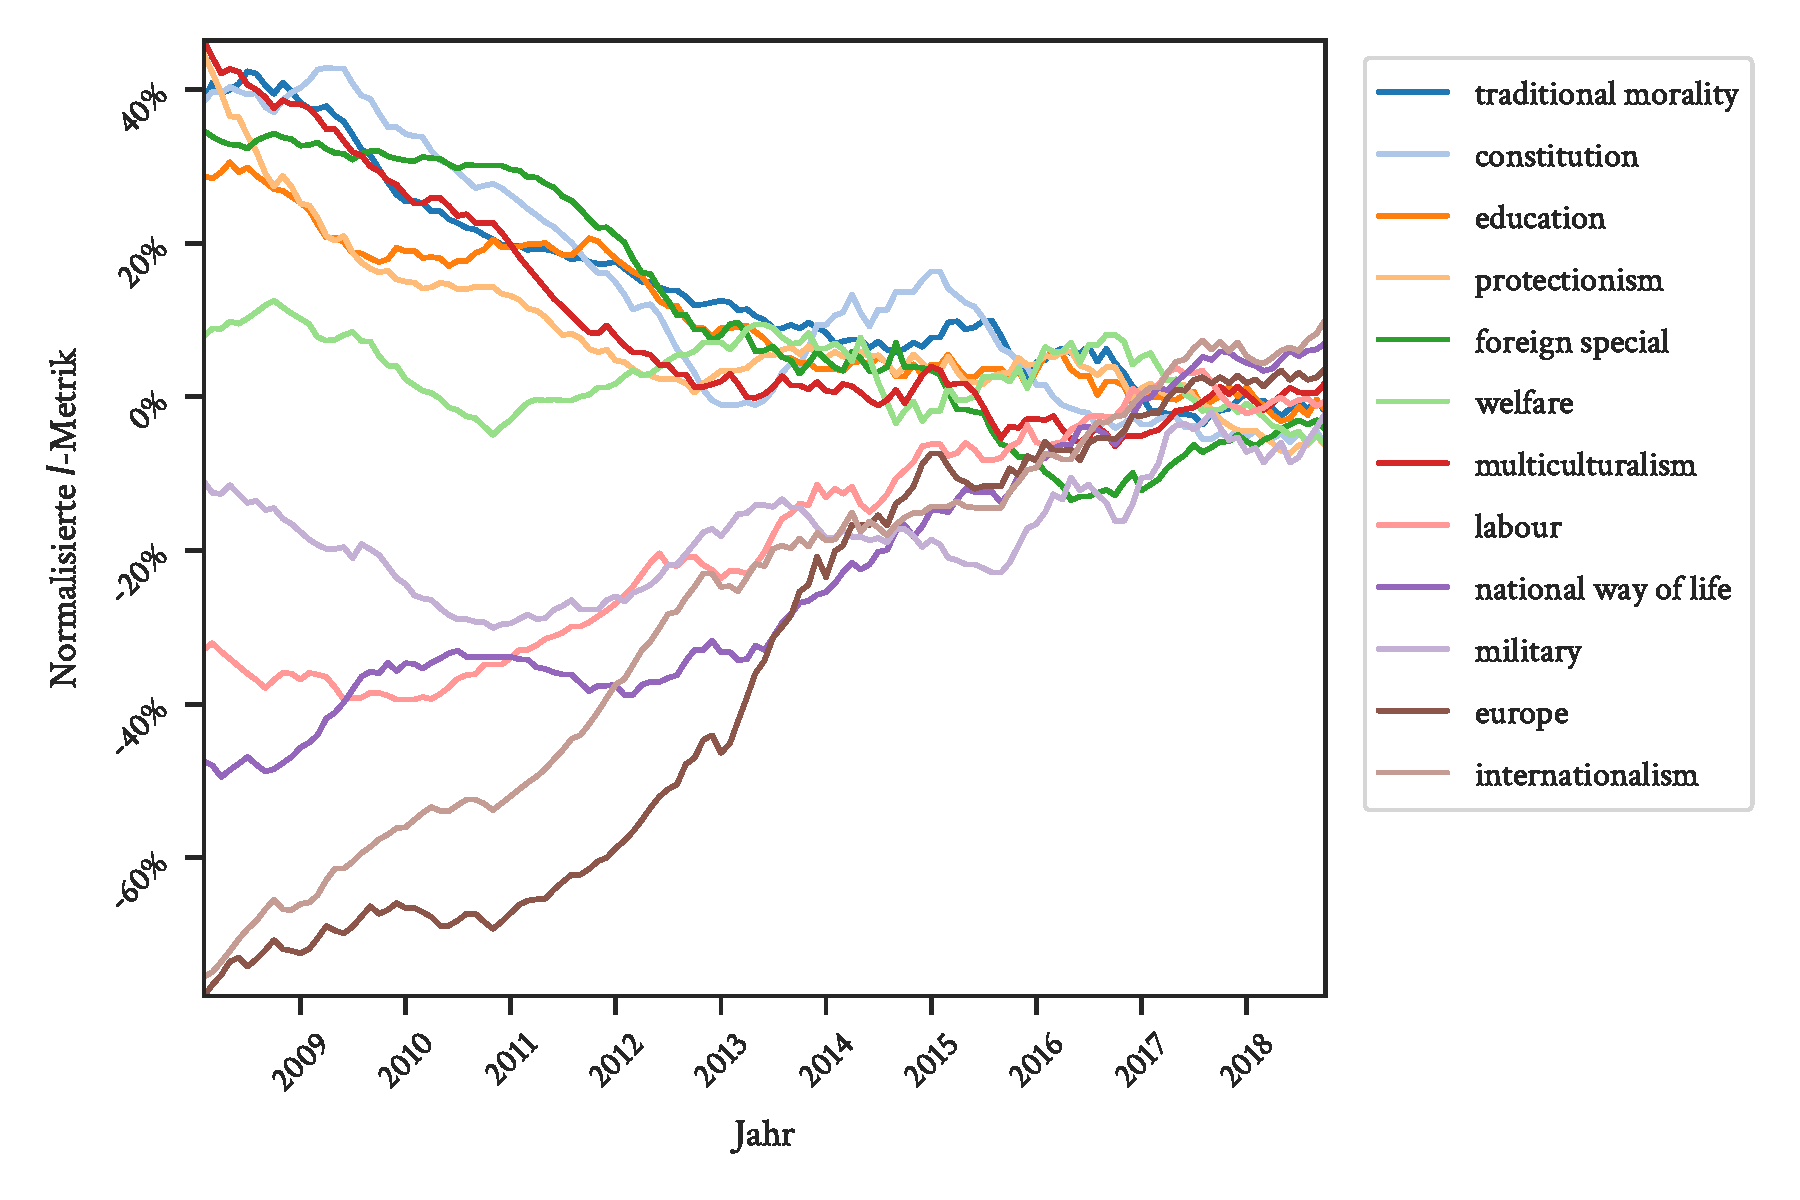
\includegraphics[width=0.9\textwidth]{./figures/lmetric_filtered_norm.pdf}
        \caption{Normalisierte \(l\)-Metriken.}
        \label{fig:5}
    \end{subfigure}
\end{figure*}

Aus \autoref{tab:3} und \autoref{fig:4} geht hervor, dass \(\l\)-Metriken in der Praxis sehr variante und größenteils kleine Werte produzieren.
Da NottDeuYTSch kein politisches Korpus ist, war dies zu erwarten -- nichtsdestotrotz lassen sich trotzdem statistisch relevante aber kleine positive und negative Korrelationen nachweisen.
Bei \(n \approx 3000000\) sind die ergebenen Korrelationen sehr präzise und ihre 95\%-Konfidenzintervalle klein.
Somit sind die Ergebnisse dieses Ansatz keine hinreichenden Belege, dass sich in der Sprache und Jugendkultur viel verändert hat, jedoch Indizien dafür, dass es tatsächlich leichte Wertetrends gab.

Beispielweise sind die Themen \emph{Europa} und \emph{Internationalismus} populärer geworden, während Themen wie \emph{traditionelle Moral}, \emph{Verfassung}, und \emph{Bildung} unbeliebter wurden.
Daraus lässt sich interpretieren, dass die deutsche Jugendkultur im Zuge der Digitalisierung auch internationalisiert wurde.
Dies wird außerdem dadurch belegt, dass der Englischanteil der deutschen Jugendsprache von 2008 bis 2020 signifikant anstieg \autocite{Po24}.

Des Weiteren deuten die leichten negativen Trends zu \emph{traditionelle Moral}, \emph{Verfassung}, \emph{Bildung}, \emph{Protektionismus} auf eine libertäre und kapitalisierende Entwicklung.
Dies lässt sich erklären dadurch, dass von 2008 bis 2018 sich neue Berufe wie YouTuber und Influencer etabliert hatten, sowie Gewinnspiele populärer wurden.
Die allgemeine Präsenz von Gewinnspielen wurde außerdem in \autoref{tab:1} festgestellt.

\subsection{Kritik} \label{subsec:3.4}
Die nur kleinen durch CorpusDiff Korrelationen ließen sich möglicherweise durch den folgenden Sachverhalt erklären.
Derzeit wird die \(l\)-Metrik als Differenz zwischen durchschnittlichen Ähnlichkeiten definiert.
Jedoch ist es möglich, dass die Einbettungen aus dem Vergleichsdatensatz, die ein gleiches Label positiv/negativ repräsentieren nicht einen konzentrierten und kreisförmigen Cluster ergeben.
Des weiteren ist es auch möglich, dass einzelne sog. \emph{Outlier}, fern von anderen Einbettungen des gleichen Labels liegen.
Wenn beides auftritt, werden nach der aktuellen Definition der \(l\)-Metrik kleine Werte produziert auch wenn eine starke relative Nähe zum jeweiligen Cluster vorliegt.

Um den zweiten Effekt zu reduzieren, sollten vorerst die Outlier gefunden und entfernt werden.
Hierfür existieren verschiedene Methoden die u.a. auch in hochdimensionalen Vektorräumen mit Winkelähnlichkeit angewendet werden können, wie \emph{angle-based outlier detection} \autocite{KSZ08}.
Alternativ berechnet HDBSCAN \autocite{MB19} auch einen sog. \emph{outlier factor} der verwendet werden kann, um Outlier zu entfernen, oder sie weniger zu gewichten in der Berechnung der \(l\)-Metrik.

Um beide Effekte zu reduzieren, könnte \(l\)-Metrik so angepasst werden, dass nicht die durchschnittlich Winkelähnlichkeit zu allen Einbettungen eines Labels berechnet wird, sondern davor das untere 25\% Quartil entfernt wird.
Das führt dazu, dass der berechnete Durchschnitt ferne Outlier eines Labels entfernt, und eher die Nähe eines nahen Teils eines Clusters berechnet.
Somit werden also entfernte Regionen eines Clusters weniger Relevant und können den Durchschnitt nicht fälschlicherweise reduzieren, wenn eine allgemeine Nähe zum Cluster vorliegt.

Eine Alternative um mit dem ersten Effekt umzugehen, wäre es nähere Einbettungen stärker im Durchschnitt zu gewichten als entferntere ohne jene vollständig aus der Berechnung zu entfernen.
Das könnte implementiert werden, indem beispielweise eine ungerade Zahl \(1 < f \in \N\) gewählt wird und die resultierende Winkelähnlichkeiten potenziert durch \(f\) werden, \(\lambda(v, u)^f\).
Um zu garantieren, dass \(\alpha_l\) zwischen \(-1\) und \(1\) liegt würde die Formel angepasst werden zu
\begin{IEEEeqnarray*}{c}
    \alpha_l: v \mapsto F\left(\frac{\sum_{u \in P_l} \lambda(v, u)^f}{2^f|P_l|}\right) - F\left(\frac{\sum_{u \in N_l} \lambda(v, u)^f}{2^f|N_l|}\right).
\end{IEEEeqnarray*}
wobei das Hinzufügen von\footnote{\(\text{sgn} : \R \rightarrow \R, x \mapsto \text{Vorzeichen von } x\).} \(F : \R \rightarrow \R, x \mapsto \text{sgn}(x) \cdot \sqrt{|x|}\) und \(2^f\) wieder \(\alpha_l\) zu \([-1, 1]\) normalisiert.

Da diese methodischen Optimierungen erst während des Schreibprozesses gefunden wurden, konnten sie nicht zeitlich implementiert werden, jedoch wären sie wichtige Chancen, um CorpusDiff in der Zukunft zu verbessern.
Weitere Ideen und Ansätze sind in \autoref{subsec:4.1} zu finden.

\section{Fazit}
In diesem Lehrforschungsprojekt wurden drei Techniken definiert und vorgestellt, um das NottDeuYTSch-Korpus zu analysieren im Blick des Wertewandels in der deutschen digitalen Kinder- und Jugendkultur.
Während ein bag-of-words-Ansatz wenig Ergebnisse lieferte, ließen sich mittels eines NTM-Ansatzes und eines neu entwickelten Korpus-Vergleichs-Tools namens CorpusDiff Entwicklungen feststellen.
Es ging ein leichter, statistisch relevanter Trend zu einer digitalisierten, kapitalisierten und internationalisierten online-Jugendkultur hervor.

\subsection{Ausblick} \label{subsec:4.1}
Die Ergebnisse dieser Arbeit basieren größenteils auf NottDeuYTSch und PoliTweets, jedoch sollten weitere Korpus-Kombinationen mittels ausgewertet werden, sowie andere Methoden verwendet werden, um die Ergebnisse zu reproduzieren.
Weitere, nicht in dieser Arbeit verwendete Datensätze und Ansätze sind in der folgenden Liste zu finden.
\begin{description}
    \item[Qbias] \emph{Qbias} \autocite{HS23} besteht aus zwei Datensätzen, von denen der erste jeweils 21 tausend US-amerikanische Zeitschriftartikel als entweder politisch \emph{links}, \emph{mittig}, und \emph{rechts} einstuft.
        Für diese Arbeit hilft dieser Datensatz, da er mittels RoBERTa in vektorielle Form gebracht werden kann, um eine Skala zu definieren, die Texte aus NottDeuYTSch politisch einordnen kann.
        Ähnlich wie bei PoliTweets ergibt sich das Problem, dass die Sprache von US-amerikanischen Journalisten nicht der deutschen YouTube Jugendsprache gleicht.

    \item[Aksenov Et. Al.] \textcite{Aks21} verwendet einen ähnlichen Datensatz wie Qbias, nur, dass stattdessen deutsche Zeitschriftartikel gesammelt wurden.
        Ähnlich wie Qbias wurden die einzelnen Texte auf eine politische Skala gesetzt.
        Bei \textcite{Aks21} sind diese Labels \emph{links-extrem}, \emph{links}, \emph{mittig}, \emph{rechts}, \emph{rechts-extrem}.
        Somit eignet sich der Datensatz vorgestellt in \textcite{Aks21}, um ein Thema wie in dieser Arbeit zu behandeln.
        Leider wurde der Datensatz niemals veröffentlicht, weswegen er nicht verwendet wurde.
        Trotzdem könnte die Methodik der Arbeit angewendet werden, um weitere Daten zu Sammeln und mithilfe von CorpusDiff auszuwerten.

    \item[LLM-basiert Analyse] Eine weitere Methode, die verwendet werden kann um massive Korpora auszuwerten, ist die Analyse mithilfe von \emph{large language models} LLM wie \emph{ChatGPT}\footnote{\url{https://chatgpt.com/}} oder einer lokalen Alternative wie \emph{Qwen3.8} \autocite{Qi26}.
        LLMs können beispielweise für NTM verwendet werden wie in \emph{TopicGPT} \autocite{Pham24}.

        Ein ähnlicher Ansatz wäre es ein LLM zu verwenden, um jedem Kommentar einen numerischen Wert für verschiedene Werte zuzuordnen.
        Dies wäre mit \emph{pplx-decider}\footnote{\url{https://ollama.com/library/pplx-decider}}, einer Variante von Qwen3.8, vergleichsweise leicht zu implementieren.

        Ein Nachteil einer LLM-gestützten Methode wäre, dass sie weitaus viel mehr Rechenzeit und Energie benötigen würde, als alle anderen vorgestellten Methoden.

    \item[Anpassung der \(l\)-Metrik] Siehe \autoref{subsec:3.4}.

\end{description}

\printbibliography[heading=bibintoc]

\section*{Anhang}\addcontentsline{toc}{section}{Anhang}
Die Quelldateien zu diesem Lehrforschungsprojekt ist unter \url{https://github.com/CrazyDiamond-75/CorpusDiff} zu finden.

Der Programmcode wurde auf einem Arch Linux System getestet mit 32 Gigabyte RAM, 100 Gigabyte Swapspace, einer RX 3700 XTX GPU, und einer Ryzen 9 5950X CPU.

Beim Erstellen dieser Hausarbeit wurde generative KI nur im Zuge des Probelesens des Textes und der Überarbeitung des Quellcodes verwendet.
\end{document}
